%+- 2 páginas
% Linguagem usada - pq? 
% Uso de metodologia:
%	Não foi usada nenhuma conhecida por causa da falta de experiência no uso de metodologias, porém foi usada uma de divisão do trabalho	
% Como foi dividido o trabalho no time?
% 	Reuniões quinzenais para definição de estratégias
%	Testes dos times com diferentes estratégias
%	Comparação com estratégias usadas anos anteriores.
%	Um responsável pelo desenvolvimento.
% 	Divisão do problema: primeiro exploração, depois exploitação, etc, etc...
% Tempo de desenvolvimento

\section{System Analysis and Design}
%an ad-hoc
For the analysis of our systems, we adopted a prototype driven approach instead of a well known software engineering methodology because the problem seemed quite simple to solve and we had no experience with them. Thus we decided that it was better to use our time developing the system than learning a methodology.

Based on the agent contest scenario description, we divided the overall problem in sub-problems, each one analysed in detail: exploration, exploitation, attack and defense, buy, repair, and inspection. A team member was engaged with programming each strategy discussed on biweekly meetings. Forty five versions of the system were produced in this phase. These versions were tested and compared with the best teams from the last contest \cite{dominic:2012,ettienne:2012,dekker:2012,behrens:2012} and also against our own versions of the system in order to select the most efficient one. In these preliminary tests, we identified some good strategies for the final implementation. To develop the SMADAS system, we spent about 500 hours, most of them testing the strategies.

The system has 20 agents of five types: repairer, saboteur, explorer, sentinel, and inspector. We considered two main distinct phases: exploration, in which the explorers identify all vertices and nodes in the map and find the best zones, and exploitation, where all agents try to conquest and defend these zones. During the match, if an agent senses a nearby enemy it calls a saboteur to attack it, and also if the agent is damaged it tries to find a repairer to be fixed. 

Our agents are able to decide their own actions, however this autonomy produces some conflicting situations like two agents deciding to exploit different zones. These situations are solved using a centralized approach, which consists of a specific agent been responsible for the group decision. For example, one of the explorers defines the zones to exploit and one of the repairers defines the reparation order. Some conflicting situations are simply prevented by using a predefined priority order among the agents, where agents with higher priorities acts before agents with less priority.

The coordination among the agents is based on two communication mechanisms: blackboard and message exchanging. The blackboard is used to provide a global graph view to the agents, since some important information about the graph structure is synchronized in it. We decided to use a blackboard because the agents need an overall view of the scenario to be able to define the system exploitation strategy. The message exchanging is used to share information about the inspected enemies, the ally agent actions and damages, and about the map zones. The communication protocol used when a damaged agent needs to be repaired is shown in Fig.~\ref{fig:protocol}. It consists of the agent asking a repairer that contacts the other repairers to find out which one is the closest to the damaged agent. Then the other repairers inform their positions and the closest one is selected to repair the damaged agent. Thus, the selected repairer will send to the damaged agent the meeting path. 


\begin{figure}
\centering 
 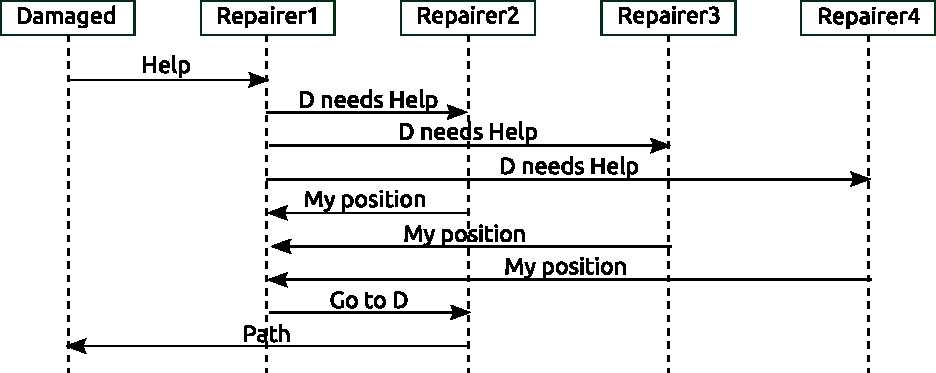
\includegraphics [width=0.9\linewidth] {./protocolo.pdf}
\caption{A communication protocol used to define which repairer will repair a damaged agent. The damaged agent asks the \texttt{repairer1} for help, the \texttt{repairer1} then contacts the others repairers to find which one is the closest to the damaged agent. All repairer send their position and the \texttt{repairer1} elects the closest one. The selected repairer then sends the meet point to the damaged agent.}
\label{fig:protocol}	
\end{figure}

The SMADAS system is a truly MAS because the agents are autonomous, reactive, and proactive. They have autonomy to decide how and when to execute most of their actions, except the few conflicting situations explained before. However, the agents also perform some actions in reaction to environment events, like the start of the step or a received message. Other reactive actions occurs when a saboteur attacks an enemy agent that is in the same vertex or when an agent runs away or defends itself from an enemy saboteur on the same vertex. Furthermore, the agents have a proactive behaviour, that shows up when they try to find a better vertex that improves the team score, contact the repairer when they are damaged, or look for enemies to attack. 

